\section[]{Embedding into Menger Sponge}
\begin{frame}{Knots Inside the Menger Sponge}
	What is a knot in the Menger Sponge?
	\begin{figure}
		\centering
		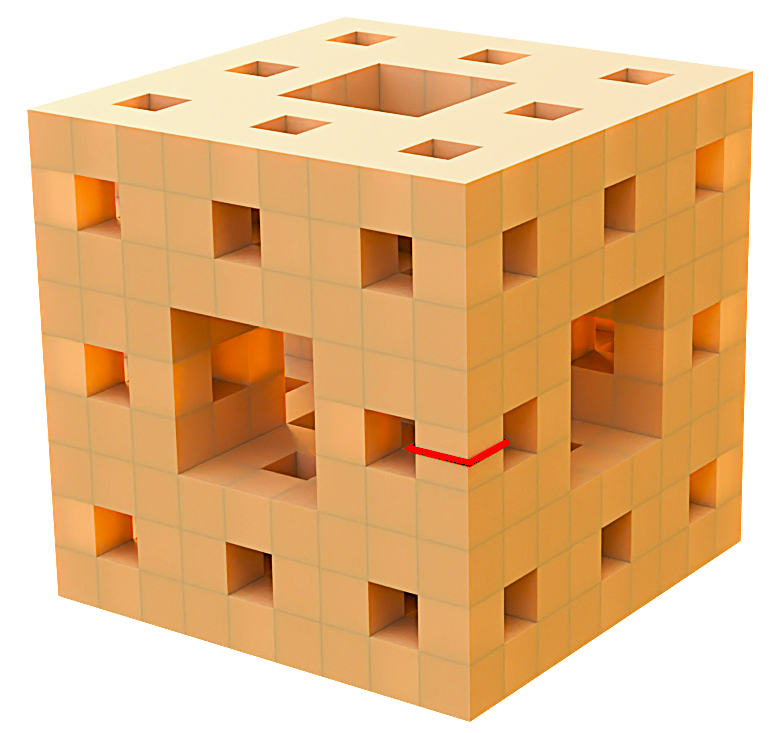
\includegraphics[width=0.35\linewidth]{UnknotTwo.png}
		\caption{The Unknot?}
		\label{fig:enter-label}
	\end{figure}
\end{frame}
\begin{frame}{Not a Knot!}
	\begin{figure}
		\centering
		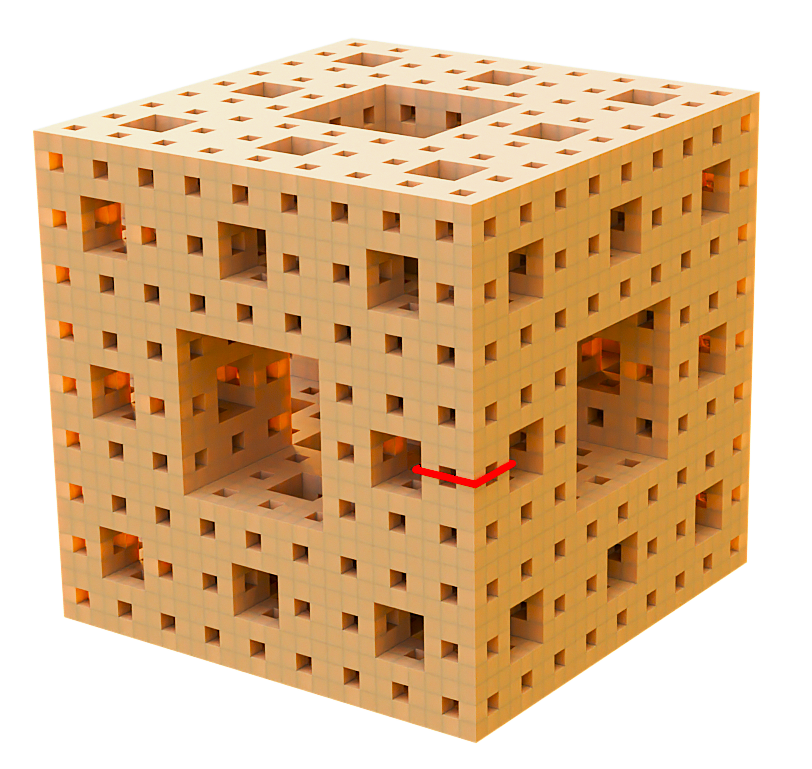
\includegraphics[width=0.49\linewidth]{NotAKnot.png}
		\label{fig:enter-label}
	\end{figure}
\end{frame}

\begin{frame}{Knot or Not?}
	\begin{itemize}
		\item Does the following knot live on the fractal?
		
		\begin{figure}
			\centering
			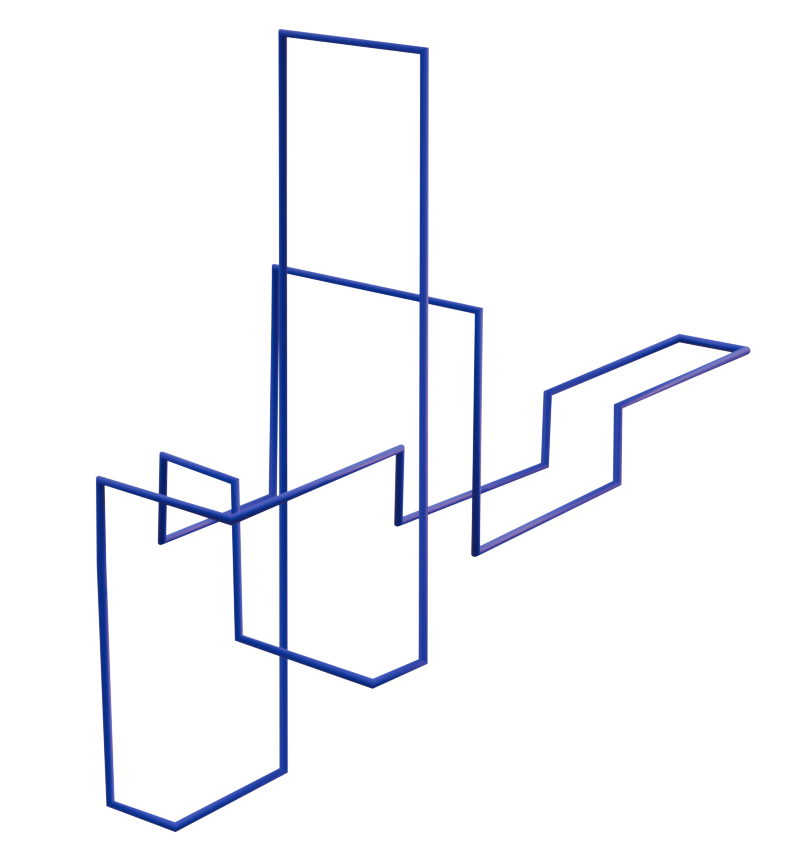
\includegraphics[width=0.25\linewidth]{NoCubeTrefoil.png}
			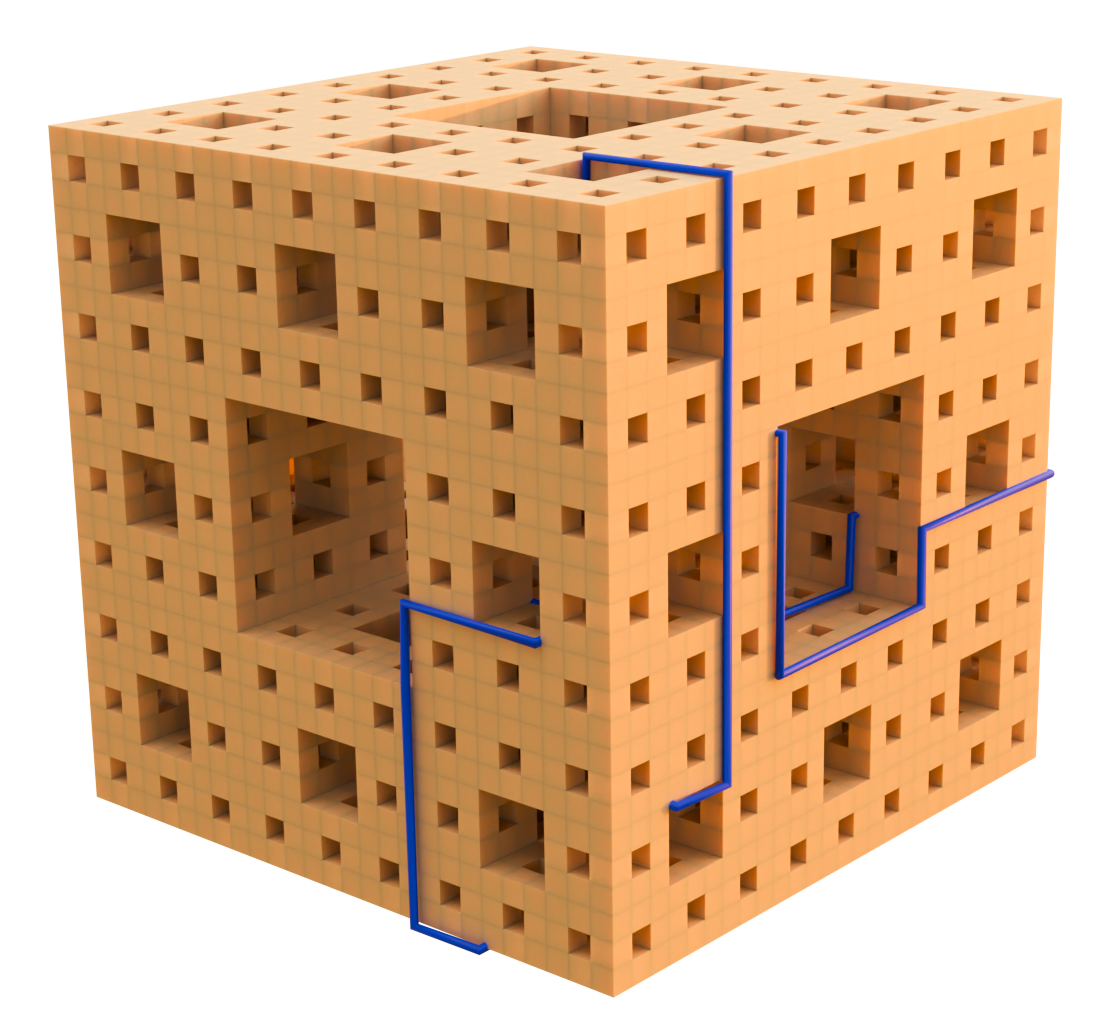
\includegraphics[width=0.3\linewidth]{TreFoilKnot.png}
			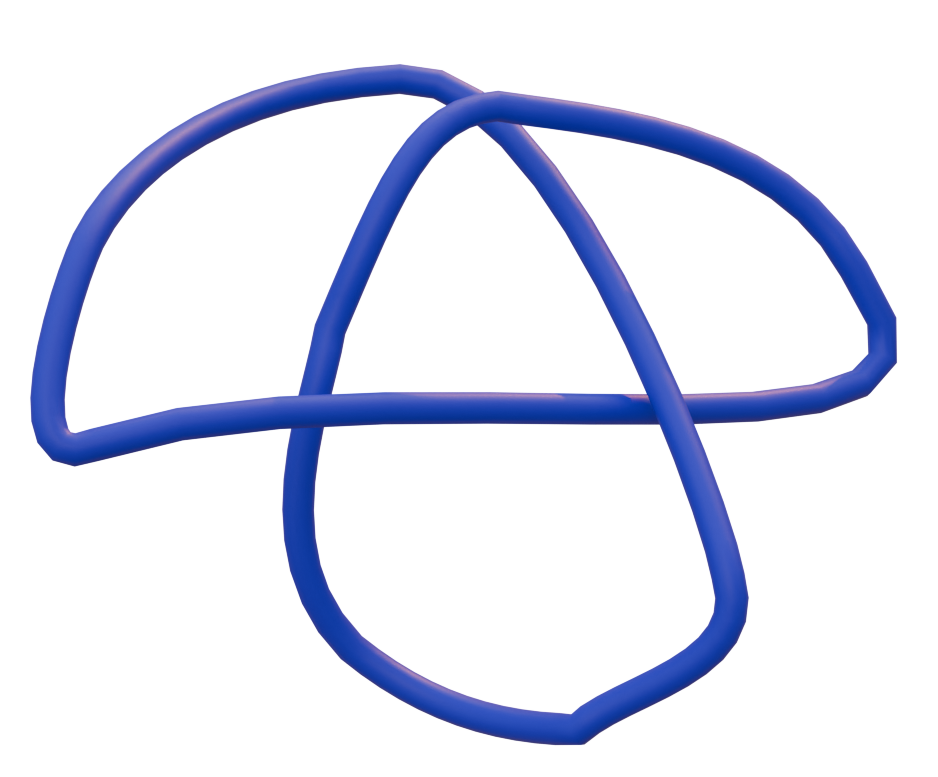
\includegraphics[width=0.3\linewidth]{UnravelledTrefoil.png}
			\caption{Enter Caption}
			\label{fig:enter-label}
		\end{figure}
		\item What possible knots can we find in this fractal?
	\end{itemize}
\end{frame}

\begin{frame}{The Positive Answer}
	\begin{center}
		This is the question asked by highschoolers Niko Voth (top right), Joshua Broden (bottom right) and Noah Nazareth under the supervision of Malors
	\end{center}
	\begin{itemize}
		\item In 2024 they were able to show that you could find every possible knot embedded in the Menger Sponge!
		\item Published a paper on ArXiv.    
	\end{itemize}
	\begin{figure}
		\centering
		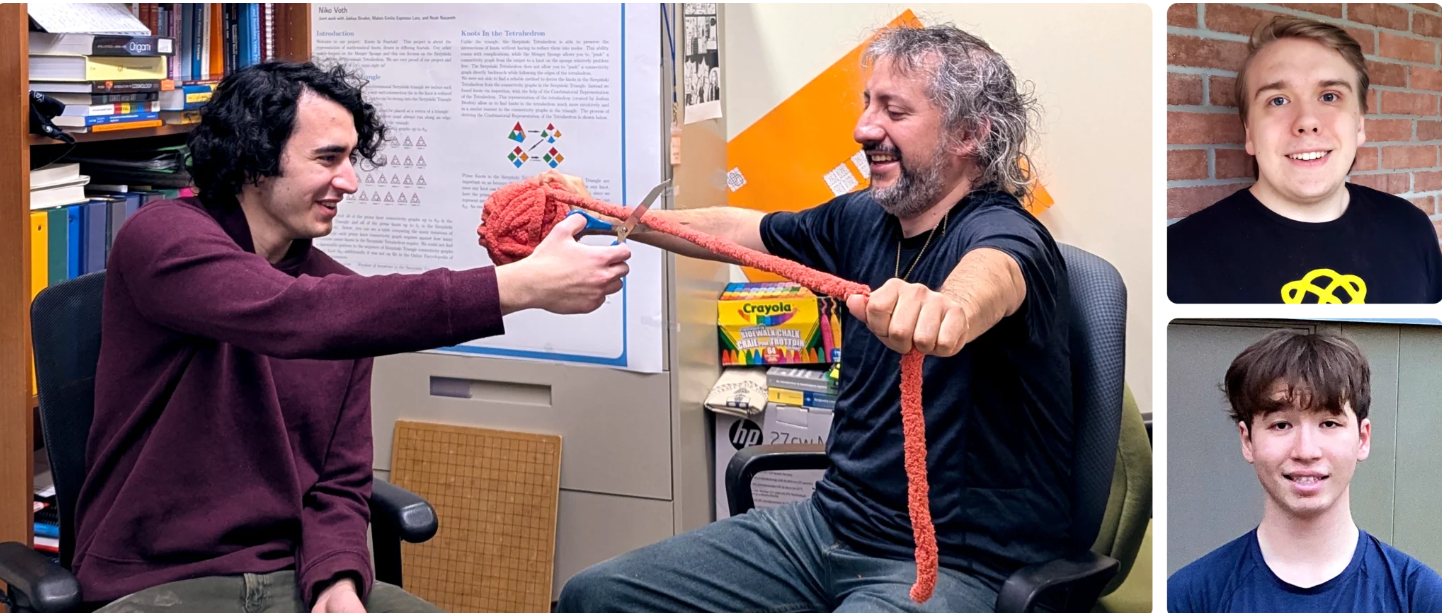
\includegraphics[width=0.5\linewidth]{PhotoOfAuthors.png}
		\caption{\cite{Quanta}}
		\label{fig:enter-label}
	\end{figure}
\end{frame}

\begin{frame}{The Cantor Set}
	\begin{itemize}
		\item Split the interval $[0,1]$ into thirds and remove the middle third
		\item Repeat on each remaining interval
	\end{itemize}
	\begin{remark}
		A point $x \in [0,1]$ is in the Cantor set if it does not have a 1 in its ternary expansion.
	\end{remark}
	\begin{figure}
		\centering
		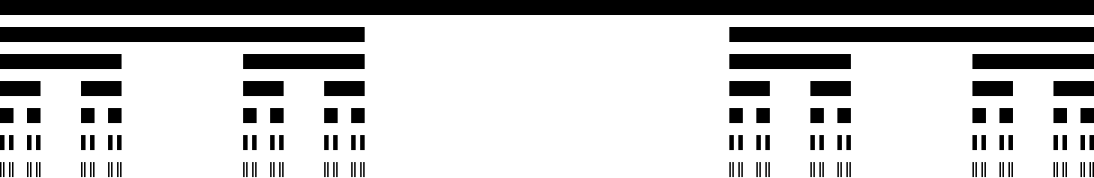
\includegraphics[width=0.5\linewidth]{Cantor_set_in_seven_iterations.svg.png}
		\caption{Cantor Set - \cite{cantor}}
		\label{fig:enter-label}
	\end{figure}
\end{frame}

\begin{frame}{Cantor Dust}
	Cantor dust is a 2 dimensional fractal and is the cartesian product of 2 cantor sets
	\begin{figure}
		\centering
		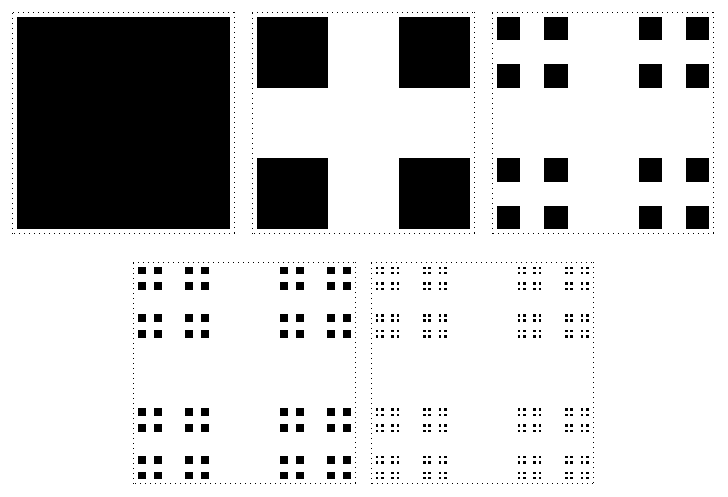
\includegraphics[width=0.5\linewidth]{cantordust.png}
		\caption{Enter Caption}
		\label{fig:enter-label}
	\end{figure}
\end{frame}

\begin{frame}{Relation With Sierpienski Carpet}
	Cantor dust is a 2 dimensional fractal and is the cartesian product of 2 cantor sets
	\begin{lemma}
		$(x,y)$ lies on the Sierpinski carpet if and only if $x$ and $y$ share no digit $1$ in their ternary expansion.
	\end{lemma}
	\begin{figure}
		\centering
		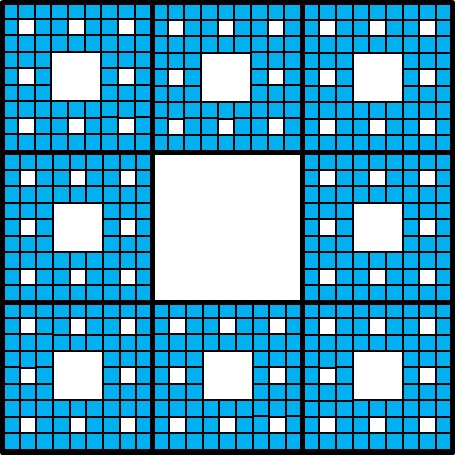
\includegraphics[width=0.2\linewidth]{Carpet.jpg}
		\caption{\cite{sierpinski2016}}
		\label{fig:enter-label}
	\end{figure}
\end{frame}

\begin{frame}{Which Points Lie on the Menger Sponge?}
	\begin{lemma}
		Let $ (x, y)$ be a Cantor Dust point, then $(x,y,z) \in M$ for all $0 \leq z \leq 1$.
	\end{lemma}
	
	\begin{proof}
		Consider the first 2 stages where regions not in black have a hole behind them. 
		\begin{figure}
			\centering
			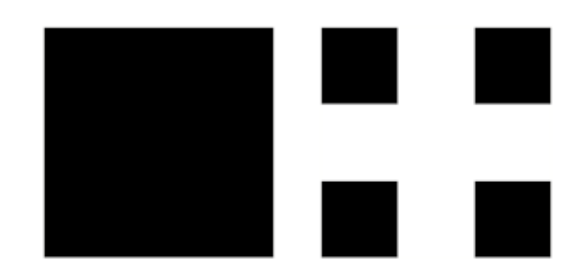
\includegraphics[width=0.22\linewidth]{ProofOfPointsOnSponge.png}
			\caption{Stage 0 and Stage 1}
			\label{fig:enter-label}
		\end{figure}
	\end{proof}
\end{frame}

\begin{frame}{Which Points Lie on the Menger Sponge?}
	\begin{proof}[Proof (Cont.)]
		\begin{itemize}
			\item In the next iteration of the sponge we need only consider the black regions as it is never possible to fill in a hole. 
			\item However, each black region occurs at a square of dimension $\frac{1}{3}\times\frac{1}{3}$ and so can be viewed as Stage $0$ when zoomed in. 
			\item Repeating this argument inductively we see that the black areas precisely align with points of the Cantor Dust fractal.
		\end{itemize}
	\end{proof}
	\begin{figure}
		\centering
		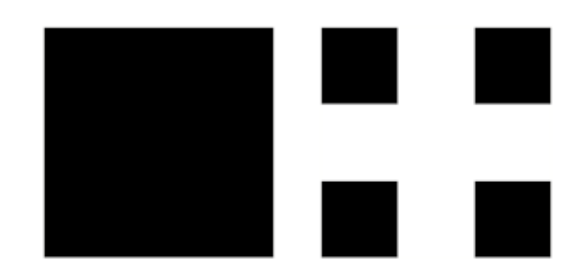
\includegraphics[width=0.22\linewidth]{ProofOfPointsOnSponge.png}
	\end{figure}
\end{frame}

\begin{frame}{Arc Presentation of Knot}
	\begin{definition}
		An Arc Presentation in grid form is an ordered list of $n$ unordered pairs
		$\{a_1, b_1\}, ..., \{a_n, b_n\}$,
		such that $a_1, ..., a_n$ and $b_1, ..., b_n$ are permutations of $1, ..., n$ and
		$a_i , b_i,$ for $ i \in \{1, ...., n\}$
	\end{definition}
	
	\begin{example}
		An Arc Presentation of the Eight Knot $4_1$ is
		\begin{center}
			$\{3, 5\}, \{6, 4\}, \{5, 2\}, \{1, 3\}, \{2, 6\}, \{4, 1\}$.
		\end{center}
		
	\end{example}
\end{frame}

\begin{frame}{Arc Presentation and Arc Index}
	An arc presentation of a link L is an embedding of L in finitely many pages of the open-book decomposition so that each of these pages meets L in a single simple arc
	\begin{figure}
		\centering
		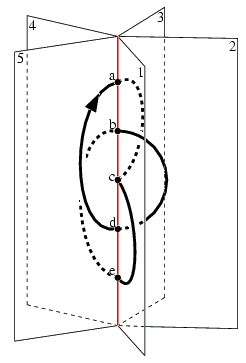
\includegraphics[width=0.2\linewidth]{MichaelImages/arc_index_fig1.png}
		\caption{Arc Presentation Trefoil}
		\label{fig:enter-label}
	\end{figure}
\end{frame}

\begin{frame}{Arc Presentation and Arc Index}
	\vspace{20px}
	\begin{definition}
		The minimum number of pages required to represent a knot is called its arc index
	\end{definition}
	
	\begin{example}
		The arc index of a $(p,q)$ torus knot is $p+q$. This was shown using techniques from contact geometry.
	\end{example}
\end{frame}

\begin{frame}[c]{Knot Game}
	\begin{center}
		Before we start the proof we will play a quick game!
		The goal is to guess the correct knot inside the sponge.
	\end{center}
	
	
\end{frame}

\begin{frame}[c]{Knots in The Menger Sponge}
	We now give the proof that every knot can be found in a finite iteration of the merger sponge.
	\begin{itemize}
		\item Given a knot $K$ we let $\{a_1, b_1\}, \dots, \{a_n, b_n\}$ be its arc presentation.
		\item Take an iteration of the Cantor set C, with at least $n$ endpoints and pick $n$ of these points $p_1, \dots p_k \in C$.
		\item We now re-write the arc presentation as $\{p_{a_1}, p_{b_1}\} \dots \{p_{a_n}, p_{b_n}\}$
		\item This does not change the knot!
	\end{itemize}
\end{frame}

\begin{frame}[c]{Knots in The Menger Sponge}
	\begin{itemize}
		\item We notice if $x_0 \in C$ then $(x_0, y,0)$ lies entirely on the front face of the sponge for $0 \leq y \leq 1$
		\item Similarly if $y_0 \in C$ $(x, y_0,0)$ lies entirely on the front face of the sponge for $0 \leq x \leq 1$
		\item We conclude the entire knot diagram induced by the given arc presentation lies on the front face of the sponge
	\end{itemize}
	
	\begin{figure}
		\centering
		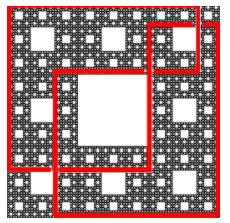
\includegraphics[width=0.2\linewidth]{KnotOnFace.png}
		\caption{Enter Caption}
		\label{fig:enter-label}
	\end{figure}
\end{frame}

\begin{frame}[c]{Push Through the Sponge!}
	The last big idea is to push the knot through the sponge
	\begin{itemize}
		\item We draw the vertical lines on the front face and the horizontal lines on the back face.
		\item We connect them through the sponge.
		\item This is possible as the points $(x_0, y_0)$ were cantor dust points!
		\item The knot is our original knot as the projection onto the front face recovers our knot diagram.
	\end{itemize}
\end{frame}